\documentclass{article}


%\usepackage[framed,numbered,autolinebreaks,useliterate]{mcode}
\usepackage{graphicx}
\usepackage{float}
%\usepackage{url}

\setlength{\parindent}{0pt}
\setlength{\parskip}{18pt}
\title{Robot Control Exercise 5: Model Predictive Control}
\author{Nicholas Shindler, \texttt{shindler25@gmail.com}}

% //////////////////////////////////////////////////

\begin{document}

\maketitle

\section{Water Tank Model}

\textit{yes, they appear to work consistently.}

\begin{figure}[H]
    \centering
    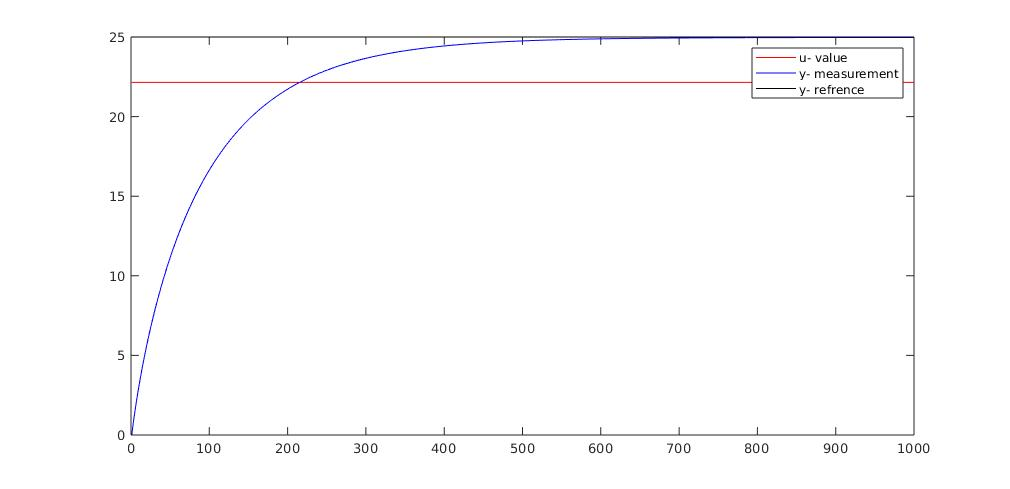
\includegraphics[width=0.6\textwidth]{wt_model_0_25.jpg}
    \caption{Test $y^r = 25$ starting from $y=0$}
    \label{fig:yr25}
\end{figure}
\begin{figure}[H]
    \centering
    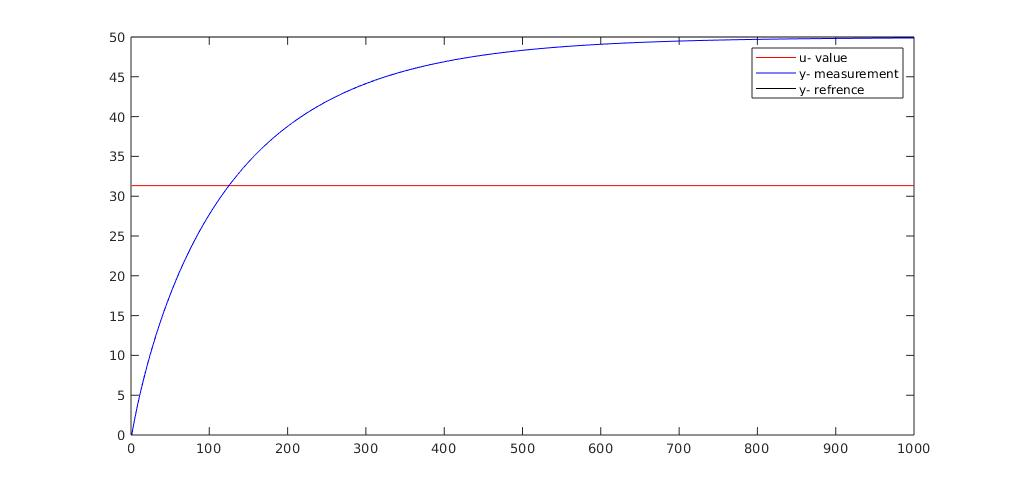
\includegraphics[width=0.6\textwidth]{wt_model_0_50.jpg}
    \caption{Test $y^r = 50$ starting from $y=0$}
    \label{fig:yr50}
\end{figure}
\begin{figure}[H]
    \centering
    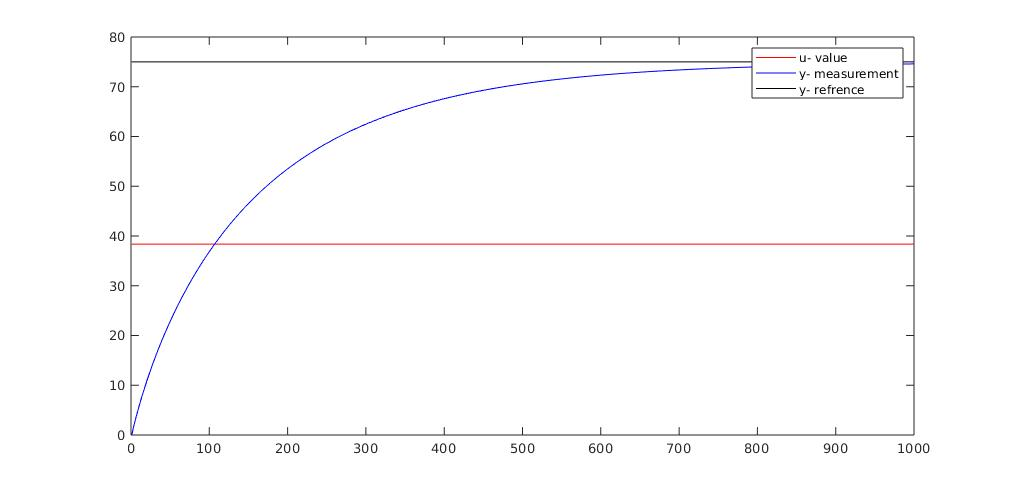
\includegraphics[width=0.6\textwidth]{wt_model_0_75.jpg}
    \caption{Test $y^r = 75$ starting from $y=0$}
    \label{fig:yr75}
\end{figure}


\begin{figure}[H]
    \centering
    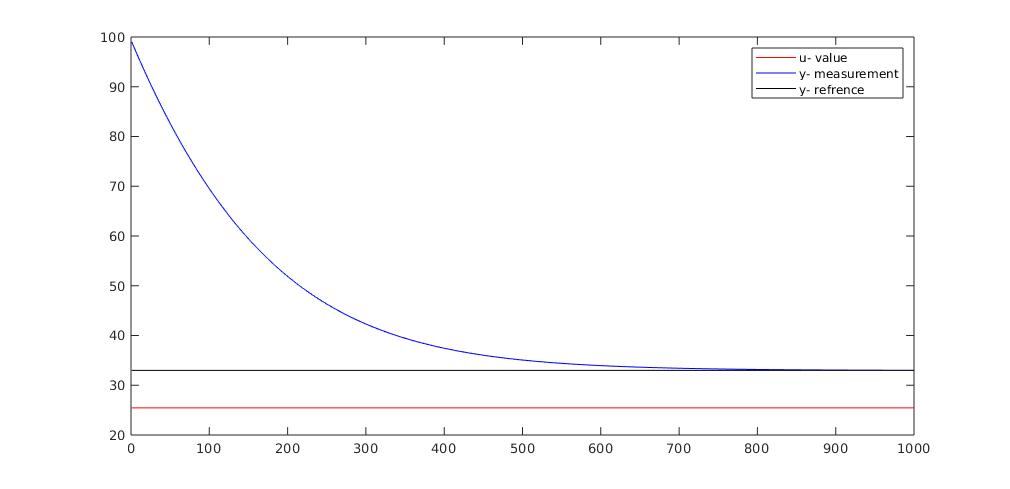
\includegraphics[width=0.6\textwidth]{wt_model_99_33.jpg}
    \caption{Test $y^r = 33$ starting from $y=99$}
    \label{fig:yisyr}
\end{figure}

\textit{Setting $y$ equal to $y^r$ results in no change.}
\begin{figure}[H]
    \centering
    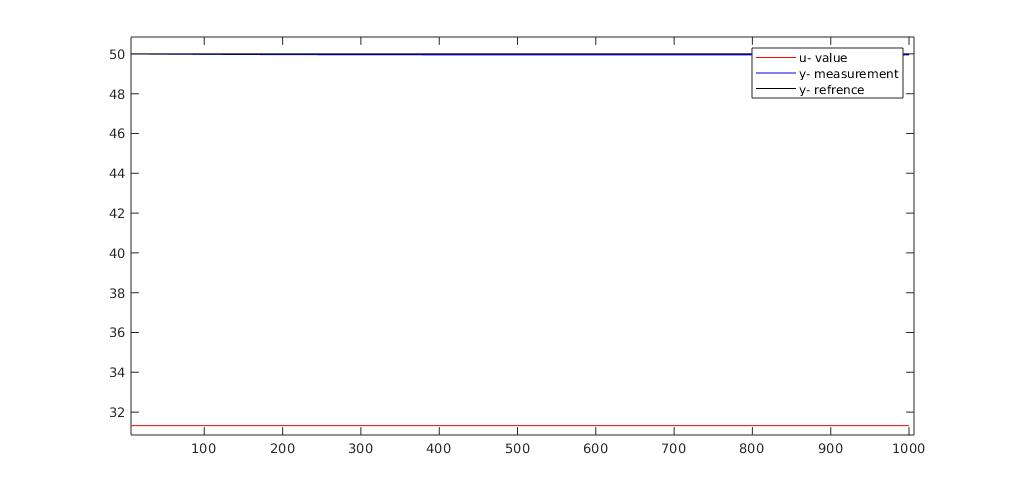
\includegraphics[width=0.6\textwidth]{wt_model_50_50.jpg}
    \caption{Test $y^r = 50$ starting from $y=50$}
    \label{fig:yisyr}
\end{figure}

\section{The MPC Formulation}

\begin{figure}[H]
    \centering
    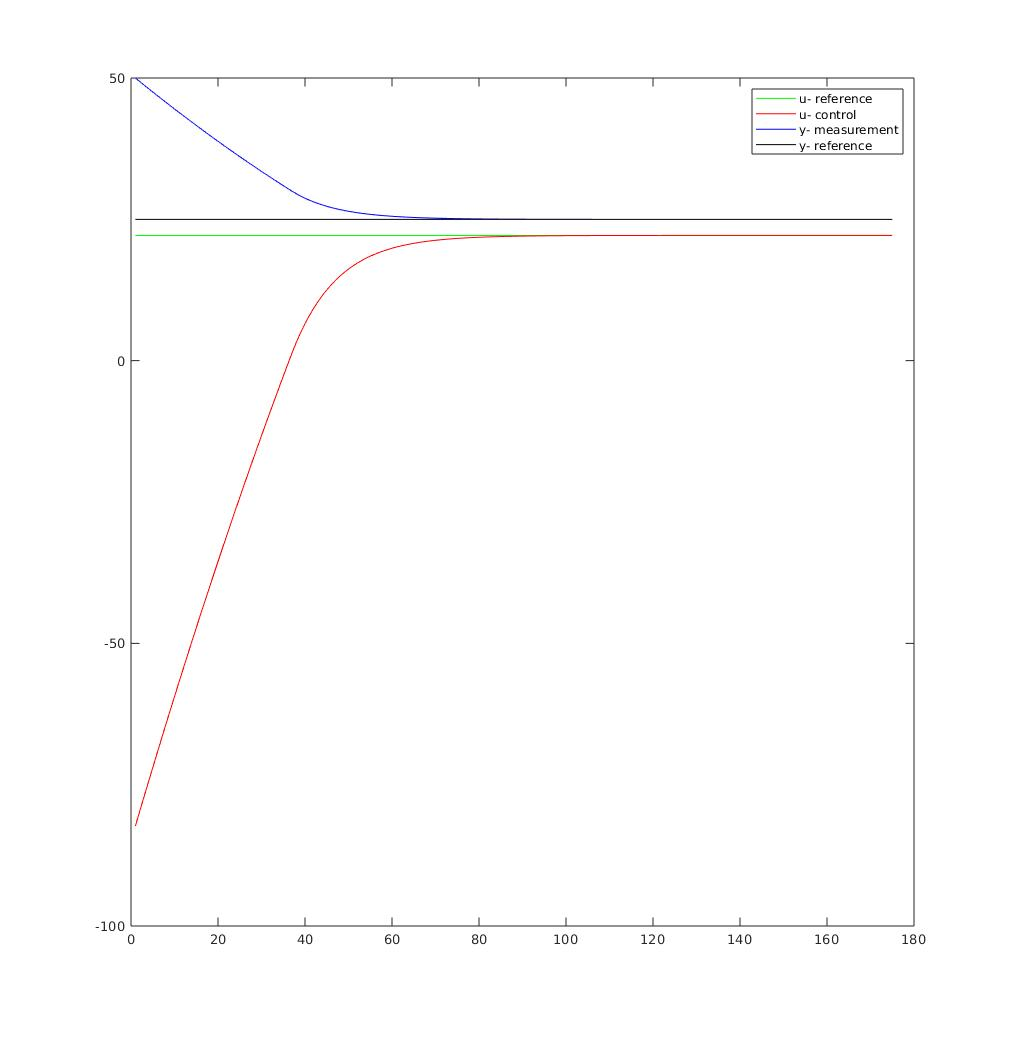
\includegraphics[width=0.4\textwidth]{yr_25_uss.jpg}
    \caption{Test $y^r = 25$ starting from $y=50$}
    \label{fig:yr25}
\end{figure}
\begin{figure}[H]
    \centering
    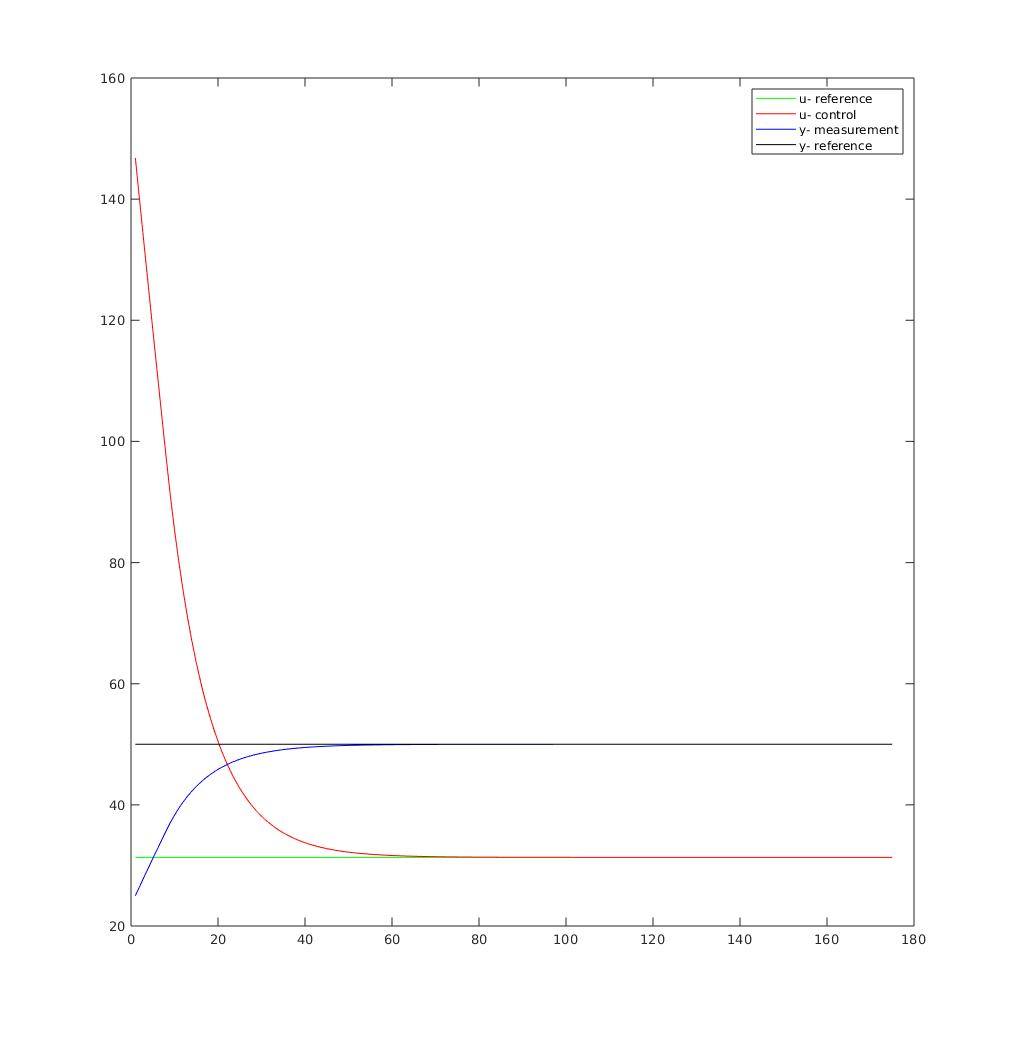
\includegraphics[width=0.4\textwidth]{yr_50_uss_25.jpg}
    \caption{Test $y^r = 50$ starting from $y=25$}
    \label{fig:yr50}
\end{figure}
\begin{figure}[H]
    \centering
    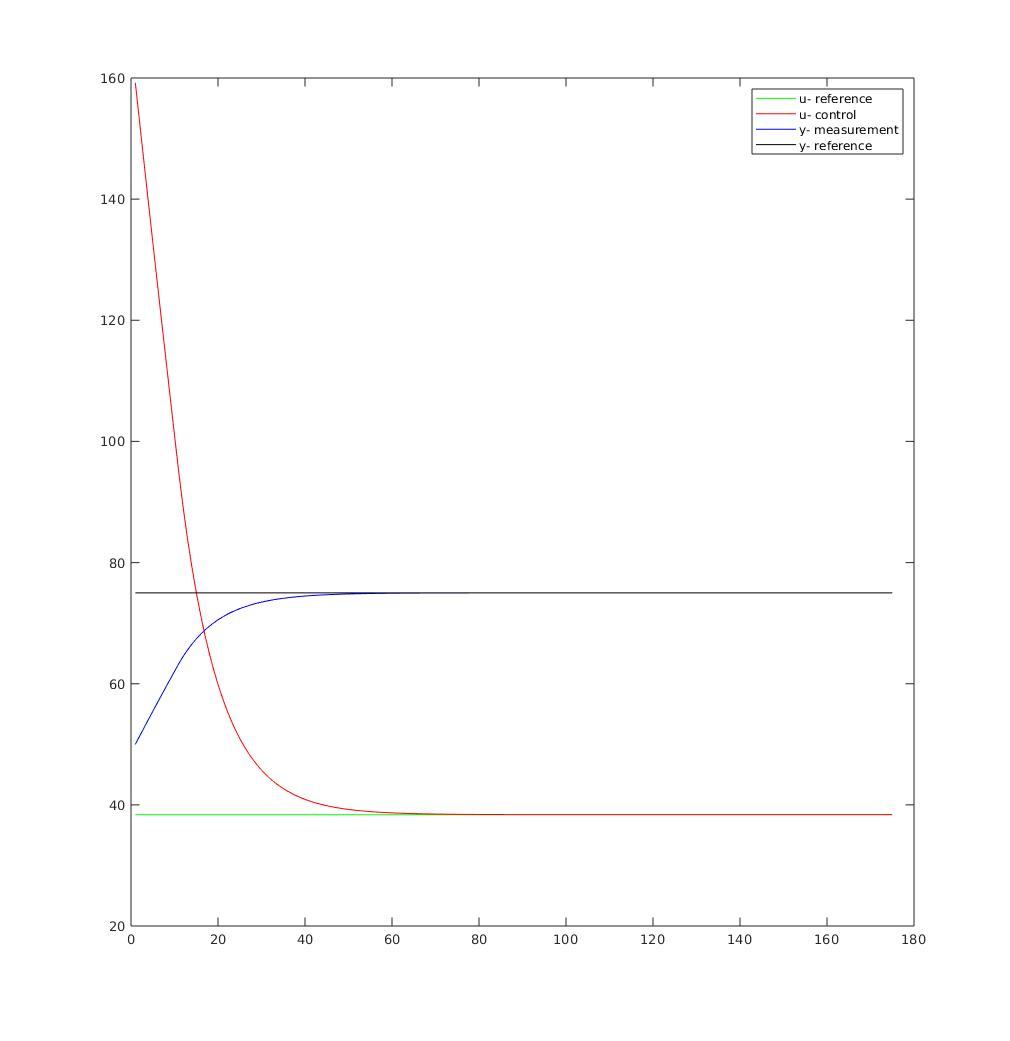
\includegraphics[width=0.4\textwidth]{yr_75_uss.jpg}
    \caption{Test $y^r = 75$ starting from $y=50$}
    \label{fig:yr75}
\end{figure}

\textit{Setting $y$ equal to $y^r$ results in no change.}
\begin{figure}[H]
    \centering
    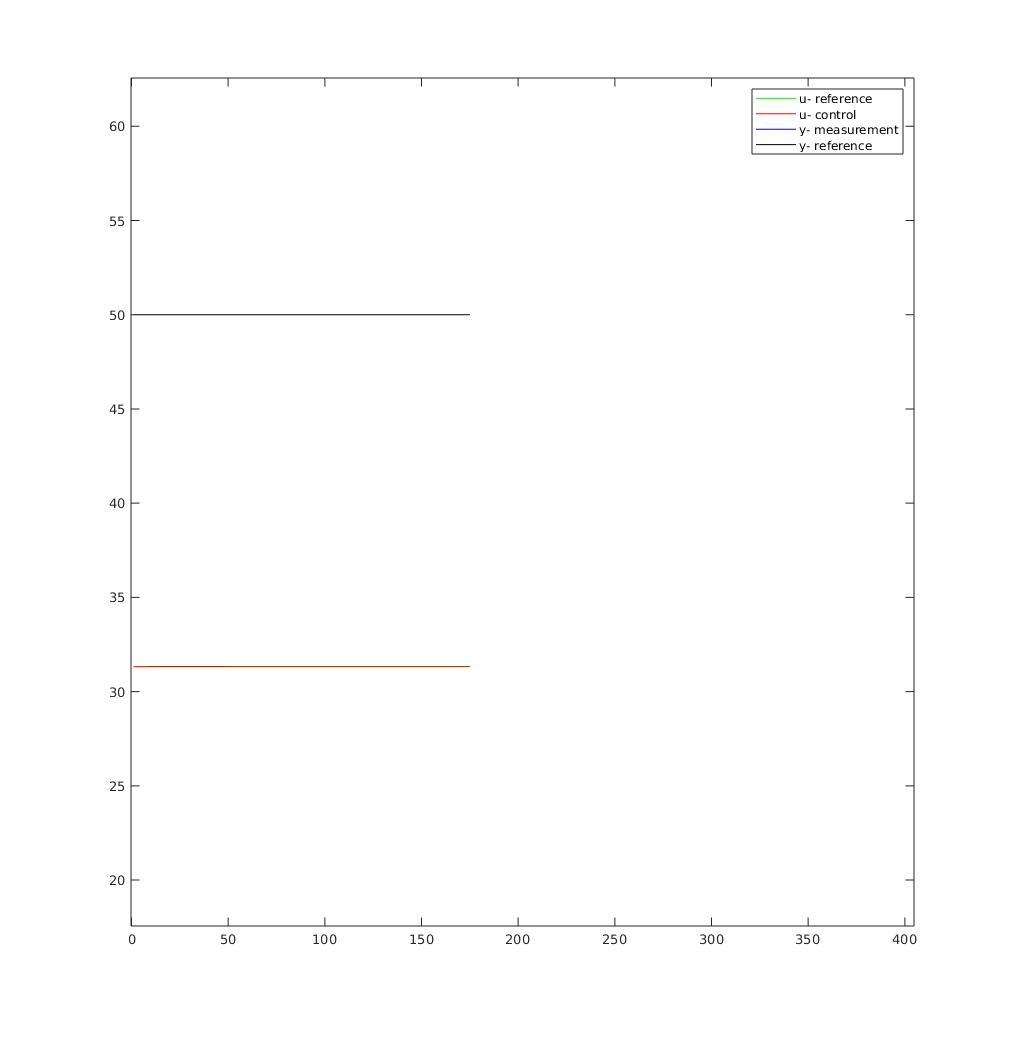
\includegraphics[width=0.4\textwidth]{yr_50_uss_50.jpg}
    \caption{Test $y^r = 50$ starting from $y=50$}
    \label{fig:yisyr}
\end{figure}

\section{MPC reference trajectory}

\subsection{custom trajectory}
\textit{creating a trajectory based on a $f(x)=(1+\exp^{-x})^{-\alpha}$ curve}
\begin{figure}[H]
    \centering
    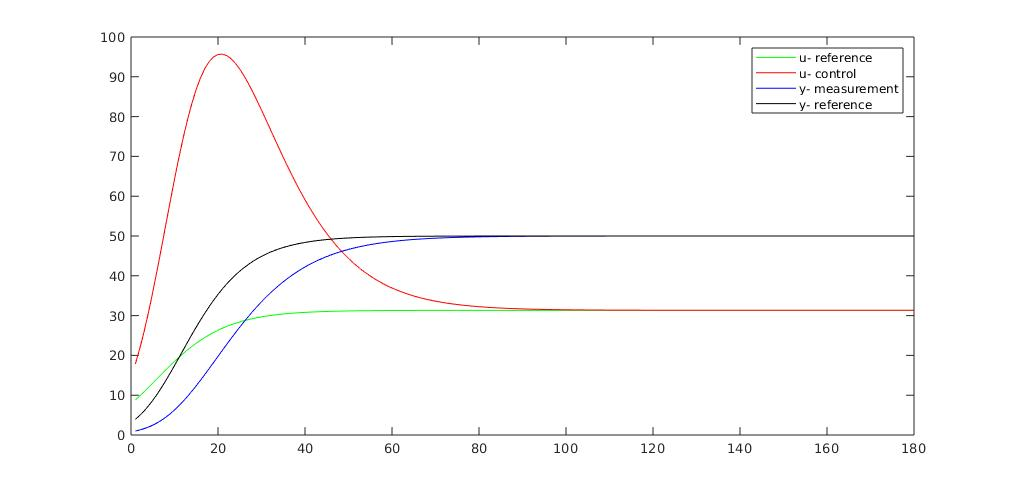
\includegraphics[width=0.9\textwidth]{mpc_trajectory.jpg}
    \caption{Test $y^r = 50$ starting from $y=0$}
    \label{fig:yr25}
\end{figure}
\begin{figure}[H]
    \centering
    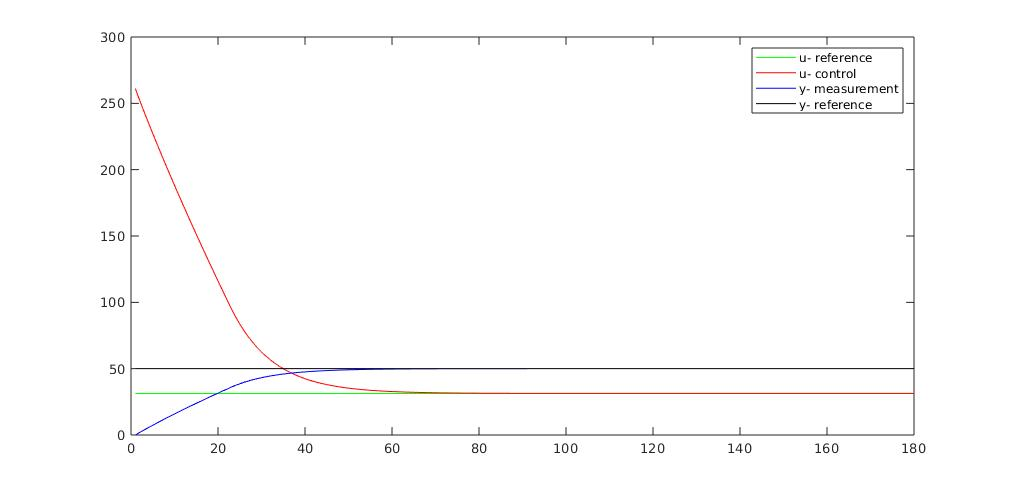
\includegraphics[width=0.9\textwidth]{mpc_default.jpg}
    \caption{Test $y^r = 50$ starting from $y=0$}
    \label{fig:yr50}
\end{figure}
This trajectory allows a much smoother curve, preventing the very high initial control values that are unnecessary as real systems are limited by physical properties and control values over a certain value are meaningless. It performed very well for what I was expecting, given how the example sin function worked.

\subsection{On - Off trajectory}

\begin{figure}[H]
    \centering
    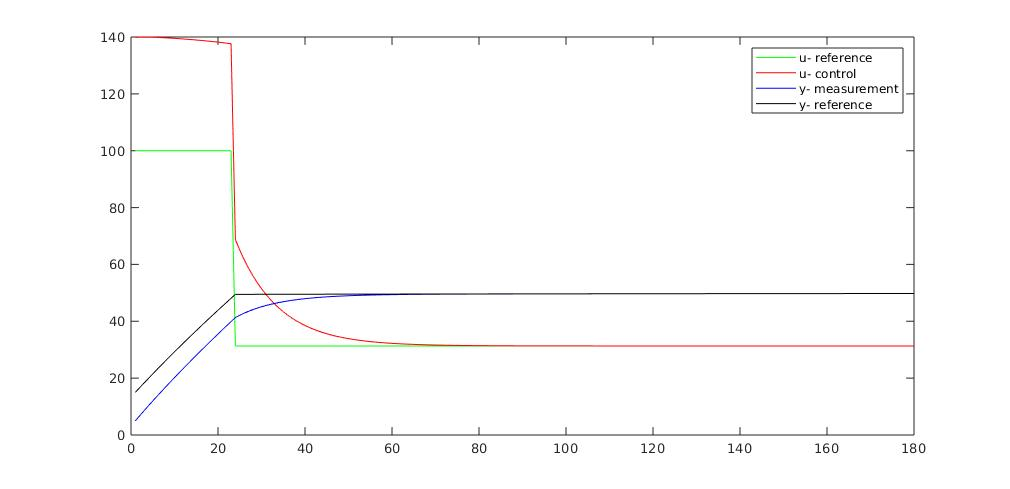
\includegraphics[width=0.9\textwidth]{mpc_on_off.jpg}
    \caption{Test $y^r = 50$ starting from $y=5$}
    \label{fig:yr50}
\end{figure}

I modified this so that at the reference point the the control would be steady state rather than 0 to prevent oscillation.
I also set the reference to start from $y=15$ rather than $y=5$ so that the reference and actual would perform slightly differently.

\subsection{PID trajectory}

This seems like a good solution when you do not know much about the system. however due to the control values it performed very similar to pure on off + steady state. Given that the on off with steady state is largely optimal as a step function this a good result.

\begin{figure}[H]
    \centering
    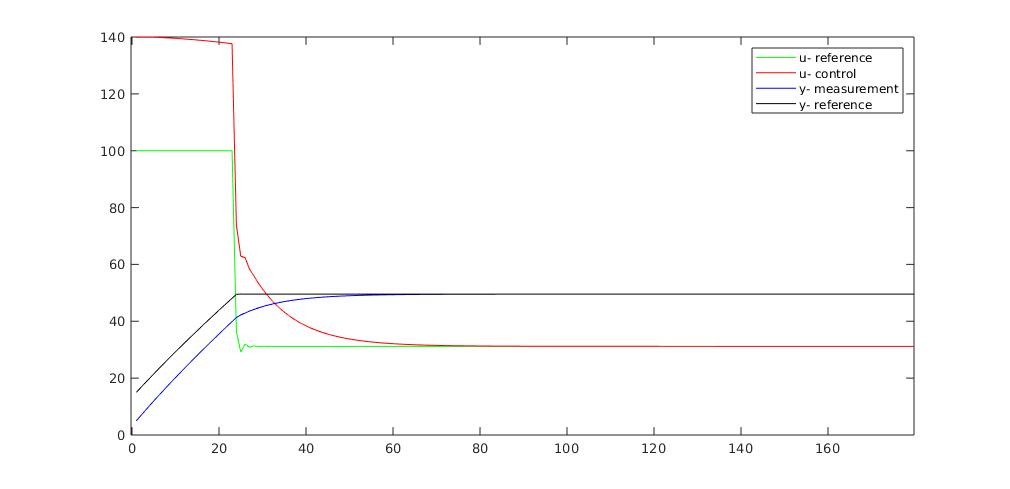
\includegraphics[width=0.9\textwidth]{mpc_pid.jpg}
    \caption{Test $y^r = 50$ starting from $y=5$}
    \label{fig:yr50}
\end{figure}

I set the reference to start from $y=15$ rather than $y=5$ so that the reference and actual would perform slightly differently.

\section{Tune the controller}

I changed A from 0.005 to 0.008, a from 0.001 to 0.0021 and $\gamma$ from 0.001 to 0.01. additionally q is scaled by 6 and r is scaled by 0.3.
I then used the trajectory function that I created for the controller.

\begin{figure}[H]
    \centering
    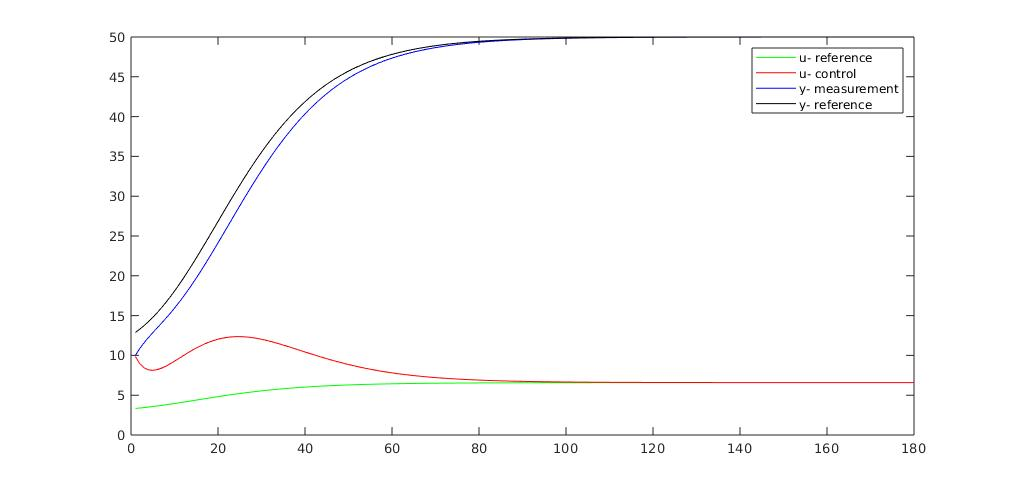
\includegraphics[width=0.9\textwidth]{mpc_modified_model.jpg}
    \caption{Test $y^r = 50$ starting from $y=10$}
    \label{fig:yr50}
\end{figure}

I further updated A from 0.005 to 0.0005, a from 0.001 to 0.0001 and $\gamma$ from 0.001 to 3 in the controller (with the model containing values as previously stated. additionally q is scaled by 42 and r is scaled by 0.7.

\begin{figure}[H]
    \centering
    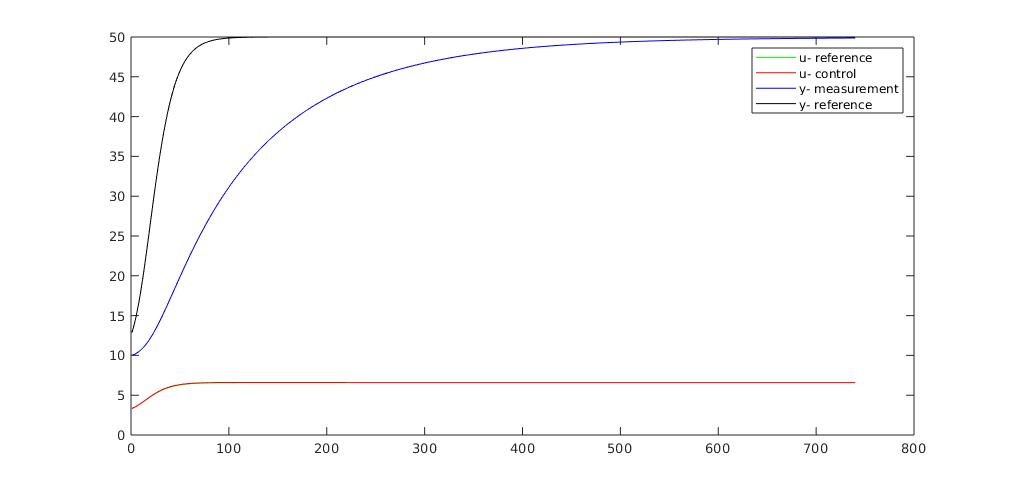
\includegraphics[width=0.9\textwidth]{mpc_heavy_modified_model.jpg}
    \caption{Test $y^r = 50$ starting from $y=10$}
    \label{fig:yr50}
\end{figure}

with these changes convergence to the set point was much slower.

I then retesting with the pid controller, which resulted in a much faster gain, though with much more noise.
\begin{figure}[H]
    \centering
    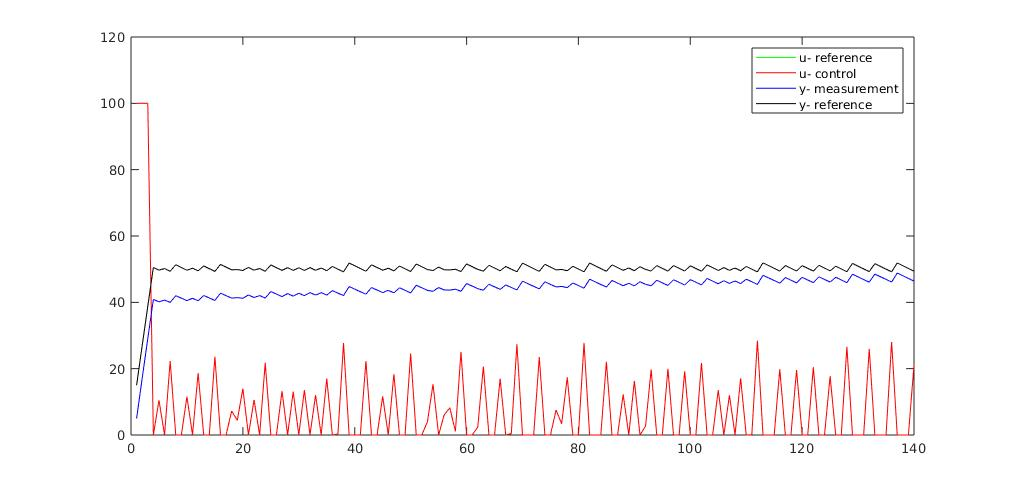
\includegraphics[width=0.9\textwidth]{mpc_heavy_modified_model_pid.jpg}
    \caption{Test $y^r = 50$ starting from $y=10$}
    \label{fig:yr50}
\end{figure}

It seemed that the scale values worked well when there  was a small error, however at large enough discrepancy between model and controller the tuning seemed to break down.

\section{Constrain the controller}

using the initial modification case I constrained to control from 0 to 30 and as a result: 

\begin{figure}[H]
    \centering
    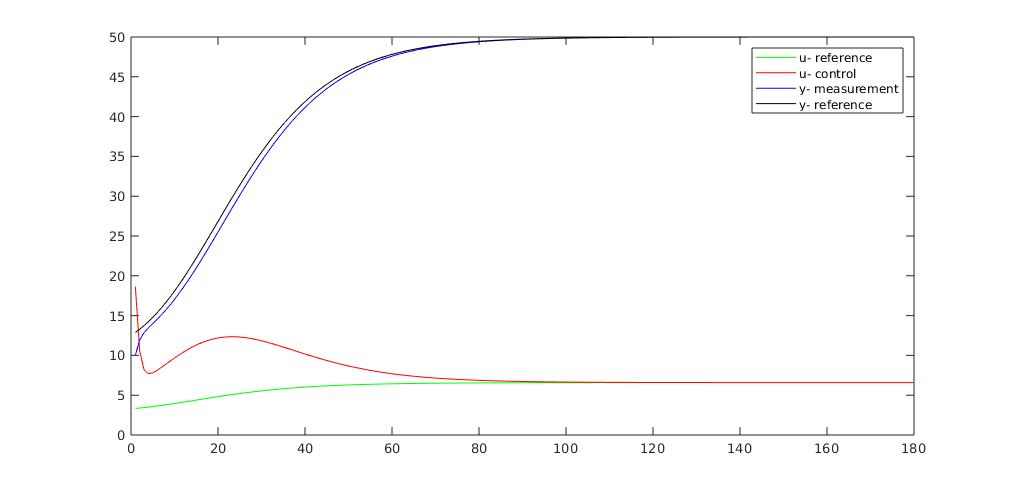
\includegraphics[width=0.9\textwidth]{mpc_modified_model_hH.jpg}
    \caption{Test $y^r = 50$ starting from $y=10$}
    \label{fig:yr50}
\end{figure}

I tested again with the steady state controller:

\begin{figure}[H]
    \centering
    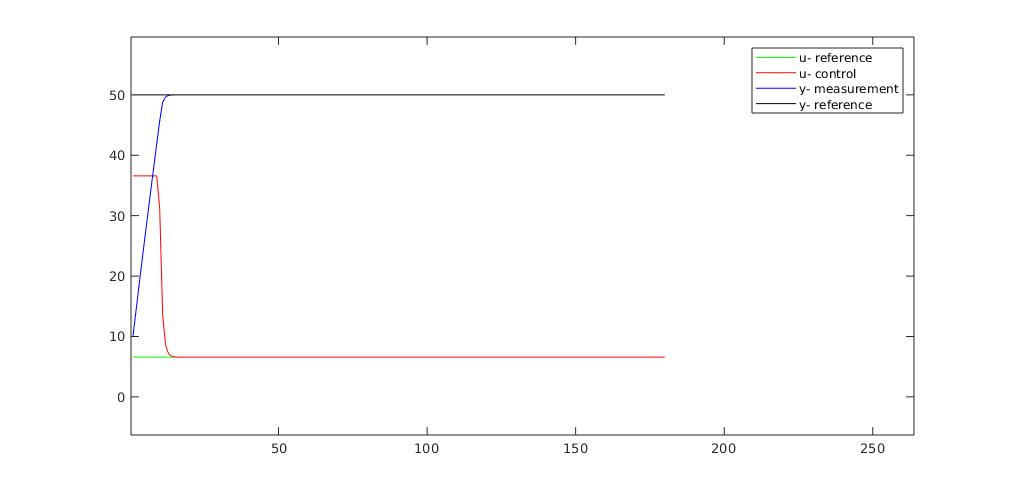
\includegraphics[width=0.9\textwidth]{mpc_modified_model_hH_ss.jpg}
    \caption{Test $y^r = 50$ starting from $y=10$}
    \label{fig:yr50}
\end{figure}

You do not see the impact of the constraints in the first case as the control is not naturally exceeding 30 however it is present in the second graph that without the limit would have a control value of about 200 to start with.

\end{document}